
\subsection{Latent variable interpretation}
\begin{frame}
 \frametitle{Proportional odds: Latent variable interpretation}
A simple motivation for the proportional odds model:
\begin{itemize}
 \item Imagine a continuous, but \emph{unobserved} response, $\xi$,
  a linear function of predictors
\begin{equation*}
\xi_i = \vec{\beta}\trans \vec{x}_i + \epsilon_i
\end{equation*}

 \item The \emph{observed} response, Y, is discrete, according to
 some \emph{unknown} thresholds,
 $\alpha_1 < \alpha_2, <\cdots < \alpha_{m-1}$
 \item That is, the response, $Y = i$ if $ \alpha_i \le \xi_i < \alpha_{i+1}$
 \item Thus, intercepts in the proportional odds model $\sim$ 
thresholds on $\xi$
\end{itemize}

\begin{center}
 \includegraphics[width=.8\textwidth]{fig/prop-odds1}
\end{center}
\end{frame}

\begin{frame}
 \frametitle{Proportional odds: Latent variable interpretation}
We can visualize the relation of the latent variable $\xi$ to
the observed response $Y$, for two values, $x_1$ and $x_2$,
of a single predictor, $X$ as shown below:
\begin{center}
 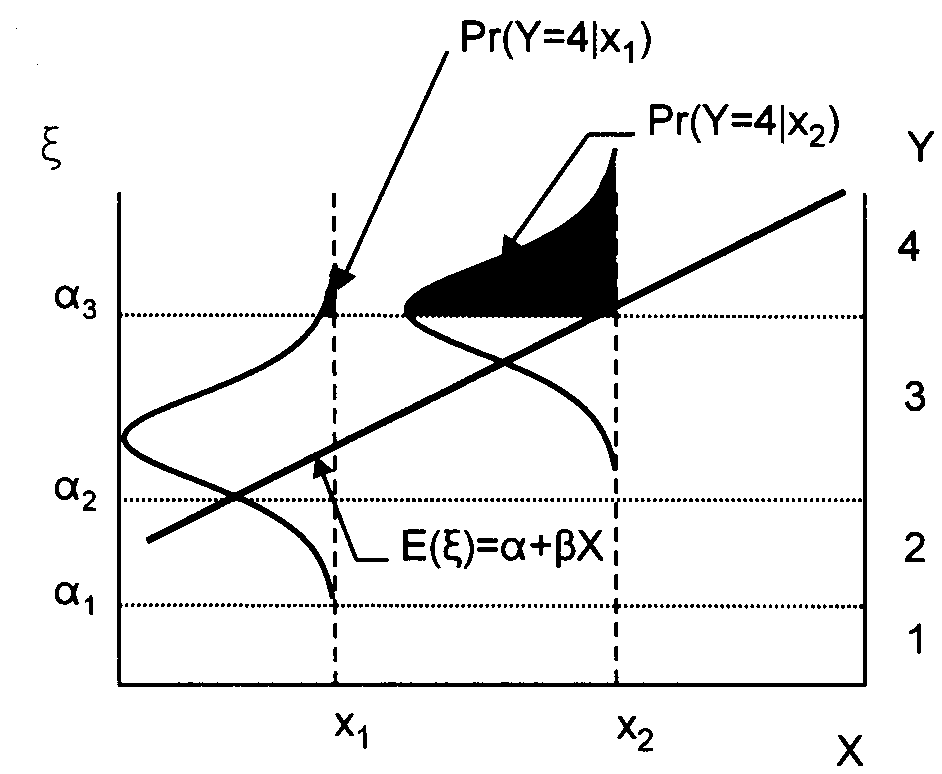
\includegraphics[width=.6\textwidth]{fig/prop-odds2}
\end{center}
\end{frame}

\begin{frame}
 \frametitle{Proportional odds: Latent variable interpretation}
For the Arthritis data, the relation of improvement to age is
shown below (using the R \pkg{effects})
\begin{center}
 \includegraphics[width=.9\textwidth]{fig/arthritis-propodds4}
\end{center}
\end{frame}
